\documentclass{template/openetcs_report}
% Use the option "nocc" if the document is not licensed under Creative Commons
%\documentclass[nocc]{template/openetcs_article}
\usepackage{lipsum,url}
\usepackage{supertabular}
\usepackage{multirow}
\usepackage{color, colortbl}
\usepackage{hyperref}
\usepackage{listings}
\usepackage{makeidx}
\definecolor{gray}{rgb}{0.8,0.8,0.8}
\usepackage[modulo]{lineno}
\usepackage{float}
\usepackage{fixme}
\usepackage{pdflscape}
\usepackage[acronym, % list of acronyms
  %section, % add the glossary to the table of content
            %description,% acronyms have a user-supplied description,
 style=longheader, % table style
 nonumberlist % no page number
  ]{glossaries}

\graphicspath{{./template/}{.}{./images/}}

\renewcommand*{\glspostdescription}{} %Deactivate point at the end of every description
\renewcommand*{\glossaryname}{Glossary}

%create glossary
% \makeglossaries
 %Glossary terms
% \loadglsentries{glossary}

\begin{document}
\frontmatter
\project{openETCS}

\newcommand{\define}[1]{\index{#1}\emph{#1}}



%Please do not change anything above this line
%============================

% The document metadata is defined below

%assign a report number here
\reportnum{OETCS/WP3/D3.5.0}

%define your workpackage here
\wp{Work Package 3: ``Modeling''}

%set a title here
\title{openETCS System Architecture and Design Specification}

%set the date of the report here
\date{May 2015}


%document approval
%define the name and affiliation of the people involved in the documents approbation here
\creatorname{Baseliyos Jacob}
\creatoraffil{DB Netz AG}

\techassessorname{Jan Welte}
\techassessoraffil{Technische Universität Braunschweig}

\qualityassessorname{Izaskun de la Torre}
\qualityassessoraffil{SQS}

\approvalname{Klaus-R\"udiger Hase}
\approvalaffil{DB Netz}


%define a list of authors and their affiliation here

\author{Baseliyos Jacob, Peter Mahlmann}
\affiliation{DB Netz AG}




% define the coverart
\coverart[width=350pt]{openETCS_EUPL}

\newpage
%define the type of report
\reporttype{Architecture and Design Specification}


\begin{abstract}
%define an abstract here
This document gives an introduction to the architecture of openETCS. The functional scope is tailored to cover the functionality required for the openETCS demonstration as an objective of the ITEA2 project. The goal is to develop a formal model and to demonstrate the functionality during a proof of concept on the ETCS Level 2 Utrecht Amsterdam track with real scenarios. It has to be read as a complement to the models in SysML and Scade languages. 
\end{abstract}

%=============================
\maketitle

%Modification history
%if you do not need a modification history table for your document simply comment out the eight lines below
%=============================


\chapter*{Modification History}
\tablefirsthead{
\hline 
\rowcolor{gray} 
Version & Section & Modification / Description & Author & Date \\\hline}
\begin{supertabular}{| m{1.2cm} | m{1.5cm} | m{4.0cm} | m{3.5cm} | m{3.5cm} |}
0.1 & Document & Initial document providing structure & Peter Mahlmann& 27.05.2015 \\\hline

\end{supertabular}

% list subsubsections in table of contents
\setcounter{tocdepth}{3}


\tableofcontents
\listoffiguresandtables
\newpage
%=============================

%Uncomment the next line if you need line numbers for tracebility when the document is in review
%\linenumbers
%=============================


% The actual document starts below this line
%=============================

\mainmatter

\chapter{Introduction}


\subsection{Motivation}
\label{sec:Motivation}

The openETCS work package WP3 aims to provide the kernel architecture and the design of the openETCS OBU software as mainly specified in UNISIG Subset\_026 version\_3.3.0. 

The appropriate functionality has been divided into a list of functions of different complexity (see \url{https://github.com/openETCS/SRS-Analysis/blob/master/System Analysis/List_Functions.xlsx}).

All these functions are object of the openETCS project and have to be analysed from their requirements and subsequently modelled and implemented. With limited manpower, a reasonable selection and order of these functions is required for the practical work that allows the distribution of the workload, more openETCS participants to join and leads to an executable---limited---kernel function as soon as possible. 

While the first version of this document focuses on the first version of the limited kernel function, it is intended to grow in parallel to the growing openETCS software.


\subsection{Objectives}
\label{sec:Objectives}



The first objective of WP3 software shall be
\begin{itemize}
	\item ``Make the train run as soon as possible, with a very minimum functionality, and in the form of a rapid prototype.''
\end{itemize}
This does not contradict the openETCS goal to conform to EN50128.
\begin{itemize}
	\item After a phase of prototyping, the openETCS software shall be implemented in compliance to EN50128 for SIL4 systems.
\end{itemize}
Additional goals for this document are
\begin{itemize}
	\item Identification of the functions required for a minimum OBU kernel
	\item Architecture overview regarding the minimum OBU kernel
	\item Technical approach: Description of the proceeding and methods to be used
	\item Road map of the minimum OBU kernel functions
	\item Road map thereafter
\end{itemize}

Note: This document will be extended according to the progress of WP3. 





\chapter{Input documents}
%-----------------------------------------------------------------------
%\subsection{Mode and Level}
%-----------------------------------------------------------------------
%\tbc
%Baseliyos Jacob
This section gives an overview about the input documents used for the
\begin{itemize}
\item analysis of the OBU functions,
\item functional decomposition and allocation of functional blocks, functions and libraries,
\item design of the OBU functions, and
\item determination of "use cases" and scenarios for the different iterations of the Architecture and Design Document
\end{itemize} 

List of main documents that are being used as reference or input for analysis and design:
\begin{itemize}
\item ERA TSI CCS documents
\item openETCS API speccification
\item openETCS requirements WP2
\item Railway operator documents
\item Industry documents
\item ERSA simulator documents
\item Other project partner data, information and documents
\item Utrecht - Amsterdam track documents
\end{itemize}

Furthermore, relevant ETCS know how from industry and operators is used for the design and the analysis.

While the list above serves as a high-level reference, detailed information, links to the actual documents and additional remarks are being maintained at
\url{https://github.com/openETCS/modeling/wiki/Input-Documents-Repository}
while the documents describing the standard are referenced at \url{https://github.com/openETCS/SSRS/wiki/SSRS-Documents}

The figure below illustrates  the relationships among the input used documents:

\begin{figure}
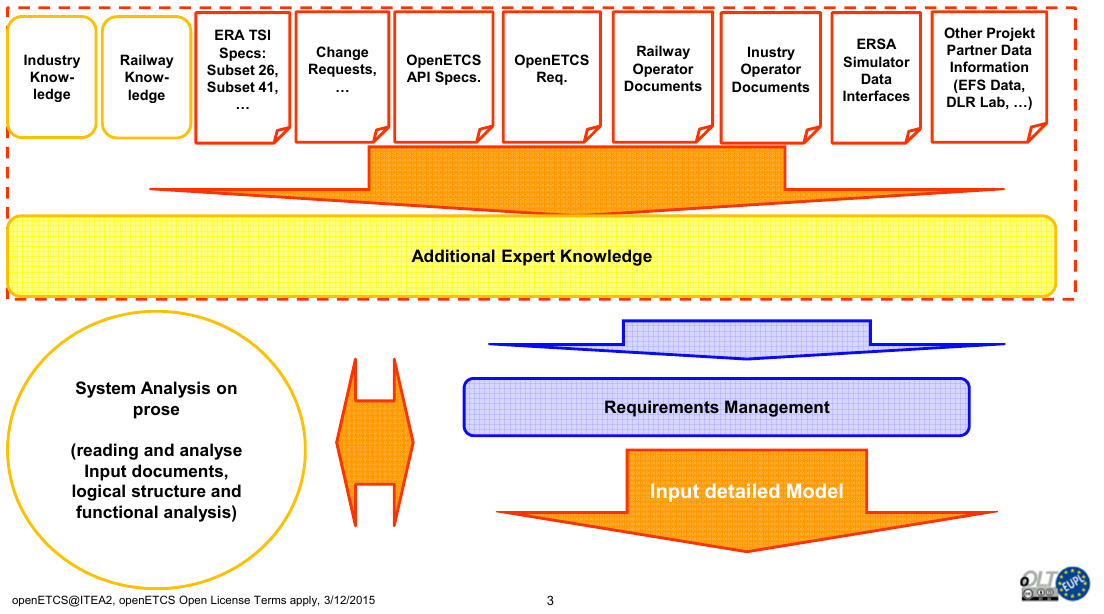
\includegraphics[scale=0.5]{images/AnalysisDocuments}
\caption{Analysis of input documents.}
\label{Analyising of input document}
\end{figure}

For a detailed discussion of the actual work process, please refer to the previous chapters. 



\chapter{Use case description - proof of concept Utrecht - Amsterdam}
%-----------------------------------------------------------------------
%\subsection{Mode and Level}
%-----------------------------------------------------------------------
%\tbc
%Baseliyos Jacob

\section{Proof of concept on the Track Utrecht Amsterdam User Stories 1 - 4}

The goal of the openETCS@ITEA2 project is to deliver at the and a proof of concept in a lab on a real ETCS Track. Since the Level 2 Utrecht - Amsterdam track was evaluated as the most approriate reference track for this concept due the maturity and representative of the track, it will be use for the mentioned simulation.\\

To start with the realisation of the concept in a iterative way in the same pattern the industry is proceeding and an regarding the "classical" state of the art of sytemanalisiys we started in this third iteration with the following Use Cases and Scenarios:\\

\subsection{Use Case and Scenario 1}
\textbf{Start of Mission - Awakening of the Train:}
This use case according to the procedure in chapter 5 will demonstrate the start of a train from a no power modus to the state that train will be ready for level and mode change according to the chapter 5.\\ 
Link on Git-Hub \url{https://github.com/openETCS/modeling/issues/66}

The following Subsystems needs to be realised for Scenario 1:\\
\begin{itemize}
\item Procedure
\item TIU Management
\item DMI Management and Controller
\item Position Report
\item Management of Radio Communication
\item Manage Track Data
\item Manage Mode and Level
\item Train Supervision
\end{itemize}

\subsection{Use Case and Scenario 2}
\textbf{Start of Mission - Start in Level 2 Mode FS:}
This use case according to the procedure in chapter 5 will demonstrate the start of a train from the awakening of the train in mode stand by to the state that train will receive a movement authority in level 2 and change into the mode full supervision to start running under real supervision according to the chapter 5.\\ 
link on Git-Hub \url{https://github.com/openETCS/modeling/issues/67}

The following Subsystems needs to be realised for Scenario 2:\\
\begin{itemize}
\item Procedure
\item TIU Management
\item DMI Management and Controller
\item Position Report
\item Management of Radio Communication
\item Manage Track Data
\item Manage Mode and Level
\item Train Supervision
\end{itemize}

\subsection{Use Case and Scenario 3}
\textbf{Brake intervention - Revocation of a Movement Authority and Overrun Permitted Speed:}
This use case according to the subset 26 chapter 3 principles will demonstrate the brake intervention that will cause by a revocation of a movement authority due to a occupied section or track an due simple overrun of a permitted speed  according to the chapter 3.\\ 
Link on Git-Hub \url{https://github.com/openETCS/modeling/issues/68}

The following Subsystems needs to be realised for Scenario 3:\\
\begin{itemize}
\item Procedure
\item TIU Management
\item DMI Management and Controller
\item Position Report
\item Management of Radio Communication
\item Manage Track Data
\item Manage Mode and Level
\item Train Supervision
\end{itemize}

\subsection{Use Case and Scenario 4}
\textbf{ETCS Onboard Unit is reading and sending track information:}
This use case according to the subset 26 chapter 3 principles will demonstrate the full completeness and checking the reading and sending of track information in interaction with the ETCS Onboard Unit and the track that will be separated in radio and balise messages. Messages and packages are defined in chapter 7 and 8 of the subset 26.\\ 
Link on Git-Hub \url{https://github.com/openETCS/modeling/issues/69}

The following Subsystems needs to be realised for Scenario 4:\\
\begin{itemize}
\item Procedure
\item TIU Management
\item DMI Management and Controller
\item Position Report
\item Management of Radio Communication
\item Manage Track Data
\item Manage Mode and Level
\item Train Supervision
\item Building of coordinate system
\end{itemize}

\section{Environment model for the use case demonstrations}

%
% nice screenshots needed!
%
%

In order to dynamically explore and demonstrate the openETCS OBU kernel software, a dynamic simulation and demonstration environmental model is being created.
During Iteration 3, this comprises the following features and functionalities:\\
•   openETCS OBU formal model \\
•   openETCS DMI formal model with Display specification model\\
•      Simplified version, not all features are implemented yet; following our use- case driven approach we are only implementing features that are essential to show the use cases selected by our "internal customer".\\
•    Environment model with \\
•  	- simplified track model (balise locations, speed profile)\\
•  	- simplified model of Movement Authority\\
•  	- interactive widgets to manipulate the simulation environment\\
\\
\\
\\


(see Figure \ref{fig:WP3-demo}.)
	
\begin{figure}
  \centering
  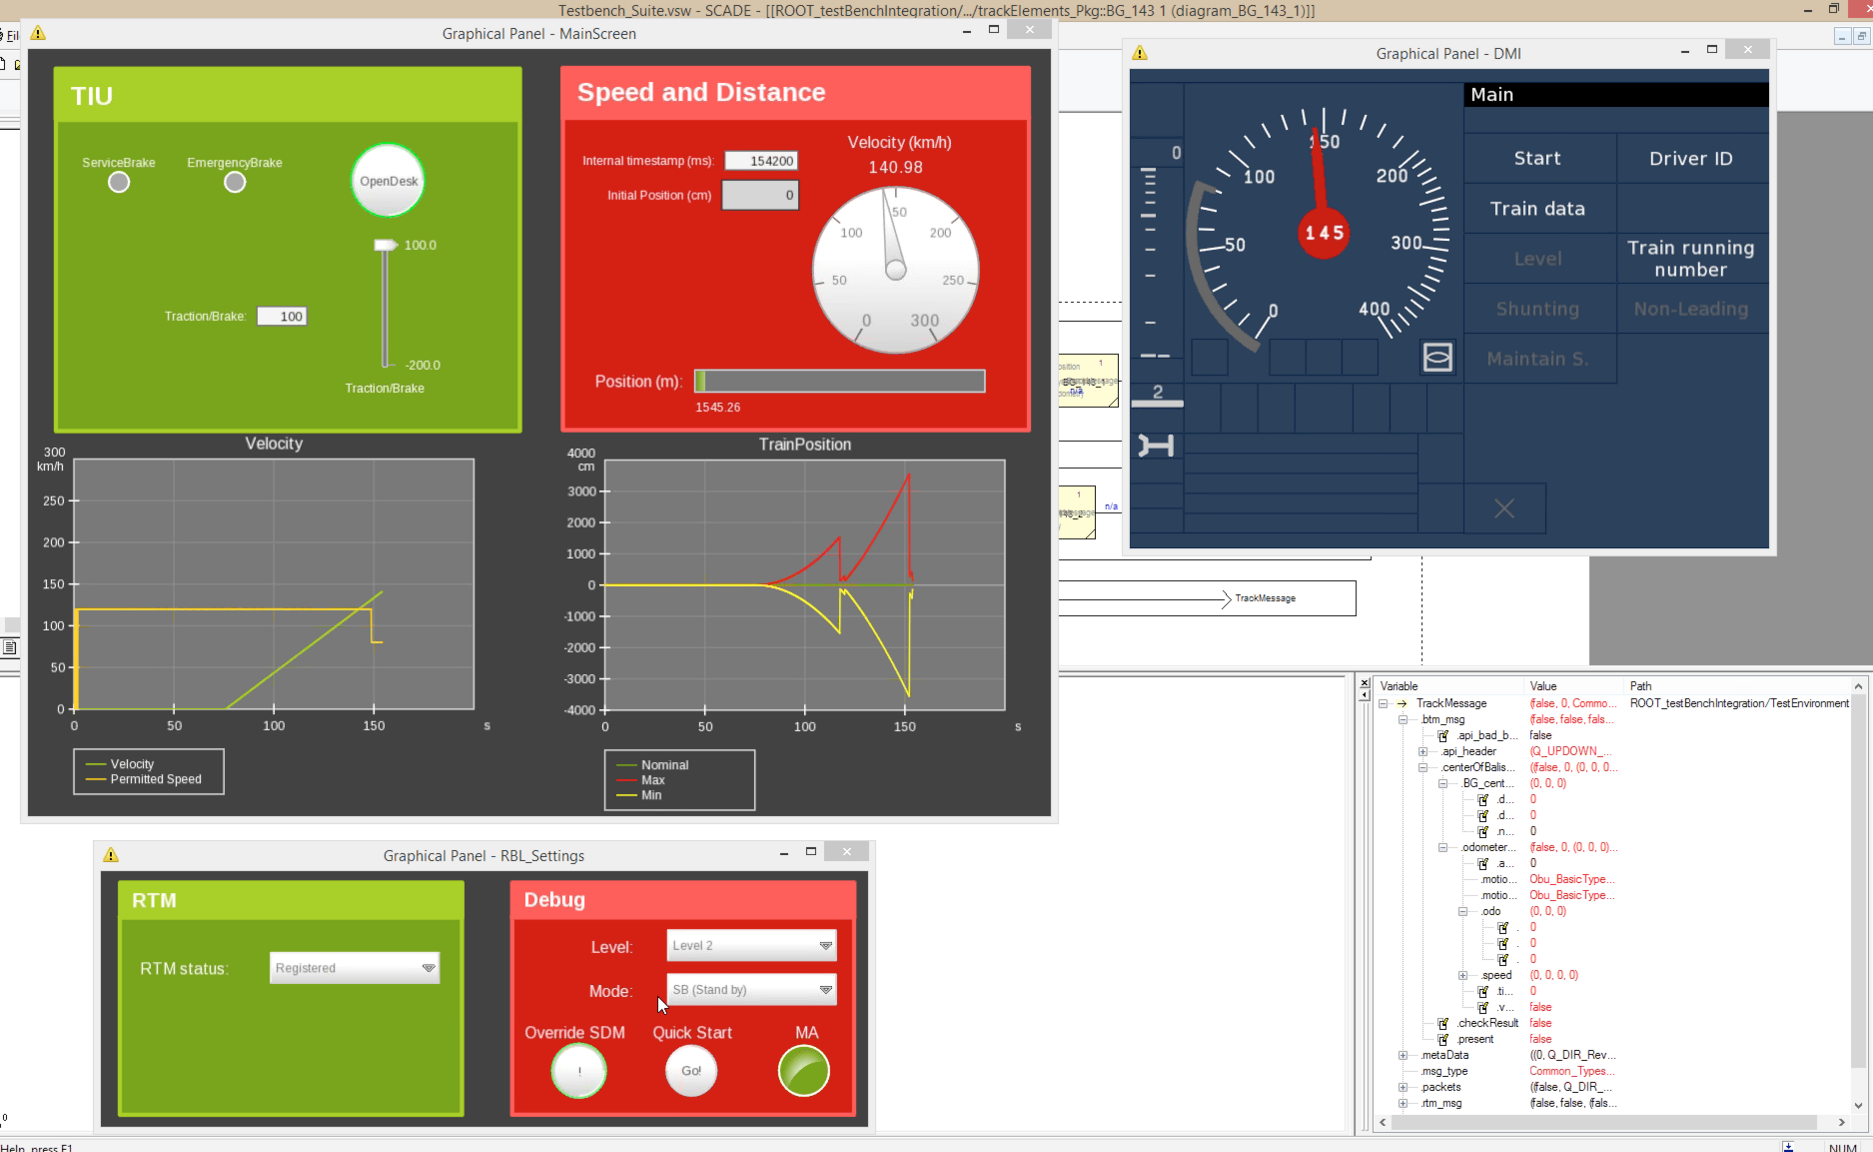
\includegraphics[width=\linewidth]{POC_environment.png}
  \caption{Environment for use case demonstration}
  \label{fig:WP3-demo}
\end{figure}




\section{Dynamic track model of the ETCS Level 2 line Amsterdam- Utrecht}

This environment model will be fourthly enhanced during the last project period, in order to:\\

•   Allow full dynamic simulation of the Utrecht- Amsterdam line\\
•   Form a basis for a (future) dynamic track simulator, which models the balise locations, balise messages and RBC messages for any given line, and which can automatically be generated from engineering datasets.\\
•   Provide a full track model for the purposes of openETCS\\
\\

(see Figure \ref{fig:track-dynamic}.)
	
\begin{figure}
  \centering
  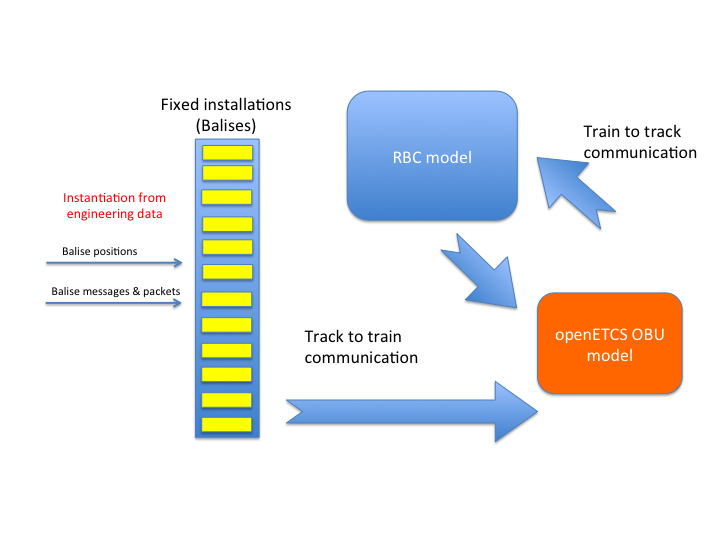
\includegraphics[width=\linewidth]{POC-track-dynamic.png}
  \caption{Schematic view of dynamic track model}
  \label{fig:track-dynamic}
\end{figure}

%
%
%
%





\chapter{Architecture Description}
%-----------------------------------------------------------------------
%\subsection{Mode and Level}
%-----------------------------------------------------------------------
%\tbc
%Baseliyos Jacob

\section{System Architecture view in ERA TSI Subset 25 Chapter 2 "Basic System Description"}
The system architecture is an outcome on the functional decomposition according to the analysis of the document in § 2 Input documents. A starting point for the first analysis is the System Strcuture in ERA TSI Subset 26 chapter 2 the subchapter 2.5 and 2.4.\\

Since we decided in the openETCS project not to consider all subsystem due to our using scope for the proof of concept on the ETCS Level 2 Utrecht - Amsterdam line, we analysed the necessary subsystem as seen here:\\

\subsection{System Structure from the subchapter 2.4. of ERA TSI Subset 26 chapter 2}

\begin{itemize}
\item 2.4.1.1	Due to the nature of the required functions, the ERTMS/ETCS system will have to be partly on the trackside and partly on board the trains. 
\item 2.4.1.2	This defines two sub-systems, the on-board sub-system and the trackside sub-system.
2.4.1.3	The environment of ERTMS/ETCS system is composed of:
\item a)	the train, which will then be considered in the train interface specification;
\item b)	the driver, which will then be considered via the driver interface specification;
\item c)	other onboard interfaces (see architecture drawing in 2.5.3),
\item d)	external trackside systems (interlockings, control centres, etc.), for which no 
\item interoperability requirement will be established.
\end{itemize}

\subsection{Sub System from the subchapter 2.5. of ERA TSI Subset 26 chapter 2}
\subsubsection{2.5.1 Trackside subsystem}
\paragraph{§ 2.5.1.1	Depending of the application level (see further sections), the trackside sub-system can be composed of:}
\begin{itemize}
\item a) balise
\item b) lineside electronic unit \textbf{\textit{- not in the scope of this project}}
\item c) the radio communication network (GSM-R)
\item d) the Radio Block Centre (RBC)
\item e) Euroloop \textbf{\textit{- not in the scope of this project}}
\item f) Radio infill unit \textbf{\textit{- not in the scope of this project}}
\item g) Key Management Centre (KMC) \textbf{\textit{- not in the scope of this project}}
\end{itemize}


\paragraph{2.5.1.2 Balise}
\begin{itemize}
\item 2.5.1.2.1	The balise is a transmission device that can send telegrams to the on-board sub-system.
\item 2.5.1.2.2	The balise is based on the existing Eurobalise specifications. These documents are included in the frame of the ERTMS/ETCS specifications.
\item 2.5.1.2.3	The balises provides the up-link, i. e. the possibility to send messages from trackside to the on-board sub-system.
\item 2.5.1.2.4	The balises can provide fixed messages or, when connected to a lineside electronic unit, messages that can be changed. 
\item 2.5.1.2.5	The balises will be organised in groups, each balise transmitting a telegram and the combination of all telegrams defining the message sent by the balise group.
\end{itemize}

\paragraph{2.5.1.3 Lineside electronic unit \textit{- not in the scope of this project}}
\begin{itemize}
\item 2.5.1.3.1	The lineside electronic units are electronic devices, that generate telegrams to be sent by balises, on basis of information received from external trackside systems.
\end{itemize}

\paragraph{2.5.1.4 Trackside radio communication network (GSM-R)}
\begin{itemize}
\item 2.5.1.4.1	The GSM-R radio communication network is used for the bi-directional exchange of messages between on-board sub-systems and RBC or radio infill units. 
\item 2.5.1.4.2	Intentionally deleted
\end{itemize}

\paragraph{2.5.1.5 RBC}
\begin{itemize}
\item 2.5.1.5.1	The RBC is a computer-based system that elaborates messages to be sent to the train on basis of information received from external trackside systems and on basis of information exchanged with the on-board sub-systems. 
\item 2.5.1.5.2	The main objective of these messages is to provide movement authorities to allow the safe movement of trains on the Railway infrastructure area under the responsibility of the RBC.
\item 2.5.1.5.3	The interoperability requirements for the RBC are mainly related to the data exchange between the RBC and the on-board sub-system.
\end{itemize}

\paragraph{2.5.1.6 Euroloop \textit{- not in the scope of this project}}
\begin{itemize}
\item 2.5.1.6.1	The Euroloop subsystem operates on Level 1 lines, providing signalling information in advance as regard to the next main signal in the train running direction.
\item 2.5.1.6.2	The Euroloop subsystem is composed of an on-board functionality and by one or more trackside parts. 
\end{itemize}
 
\paragraph{2.5.1.7 Radio infill Unit \textit{- not in the scope of this project}}
\begin{itemize}
\item 2.5.1.7.1	The RADIO INFILL subsystem operates on Level 1 lines, providing signalling information in advance as regard to the next main signal in the train running direction.
\item 2.5.1.7.2	The RADIO INFILL subsystem is composed of an on-board functionality and by one or more trackside parts (named RADIO INFILL Unit).
\end{itemize}
 
\paragraph{2.5.1.8 KMC \textit{- not in the scope of this project}}
\begin{itemize}
\item 2.5.1.8.1	The role of the KMC is to manage the cryptographic keys, which are used to secure the EURORADIO communications between the ERTMS/ETCS entities (ERTMS/ETCS on-board equipments, RBCs and RIUs).
\end{itemize}

\paragraph{2.5.2 On-board sub-system \textit{kernel part of the project}}

\textbf{2.5.2.1	Depending of the application level (see further sections), the on-board sub-system can be composed of:}
\begin{itemize}
\item a)	the ERTMS/ETCS on-board equipment;
\item b)	the on-board part of the GSM-R  radio system;
\end{itemize}


\textbf{2.5.2.2	ERTMS/ETCS on-board equipment}
\begin{itemize}
\item 2.5.2.2.1	The ERTMS/ETCS on-board equipment is a computer-based system that supervises the movement of the train to which it belongs, on basis of information exchanged with the trackside sub-system. 
\item 2.5.2.2.2	The interoperability requirements for the ERTMS/ETCS on-board equipment are related to the functionality and the data exchange between the trackside sub-systems and the on-board sub-system and to the functional data exchange between the on-board sub-system and:
\item a) the driver;
\item b) the train;
\item c) the onboard part of the existing national train control system(s).
\end{itemize}

\textbf{2.5.2.3	Onboard radio communication system (GSM-R)}
\begin{itemize}
\item 2.5.2.3.1	The GSM-R on-board radio system is used for the bi-directional exchange of messages between on-board sub-system and RBC or radio infill unit. 
\item 2.5.2.3.2	Intentionally deleted.
\end{itemize}

\paragraph{2.5.3. ERTMS/ETCS Reference Architecture}
\textit{\textbf{The figure below shows the system scope for design of the ETCS Subsystem regarding the openETCS Onboard Unit and the Test Environment within the scope of the openETCS project proof of conept on ETCS Level 2 Utrecht - Amsterdam.}}

\subsection{System Structure from the subchapter 2.4. of ERA TSI Subset 26 chapter 2}
\begin{figure}[h]
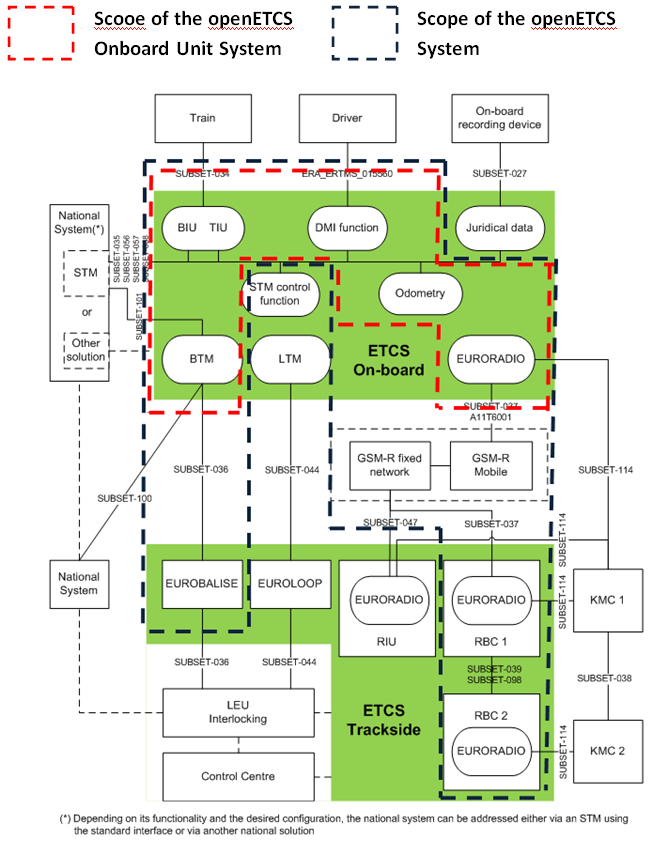
\includegraphics[scale=0.7]{images/ArchitectureSRS}
\caption{Scope of System according to ERA TSI Chapter 2}
\label{Scope of System according to ERA TSI Chapter 2}
\end{figure}

\section{System Architecture SysML View}
\textbf{The SysML System view of the architecture will reflect the scope accorgin to 4.1 and is a top down breakdown to the design layer. The functional breakdown has been done in Scade System and is part of the design model. Furthermore it will reflect all the external and internal interface that will will be described in 4.3. Another goal of the System Architecture SysML view is to explain and set the boundaries for the ETCS Kernel development "F2 Kernel" as the main design part of the openETCS@ITEA2 project.}

\subsection{1st level System Architecture view}
\textbf{All subystem of the ETCS/ERTMS Basic Sytem according in the scope of the openETCS@ITEA2 project will be reflected in this 1st level view. Furthermore the interlocking as part of a full Rail Signalling System, but not part of the openETCS scope, will be highlighted in this view.}

\textit{Interlocking =  interlocking is an arrangement of signal apparatus that prevents conflicting movements through an arrangement of tracks such as junctions or crossings. The signalling appliances and tracks are sometimes collectively referred to as an interlocking plant. An interlocking is designed so that it is impossible to display a signal to proceed unless the route to be used is proven safe.}


\begin{figure}[h]
\centering
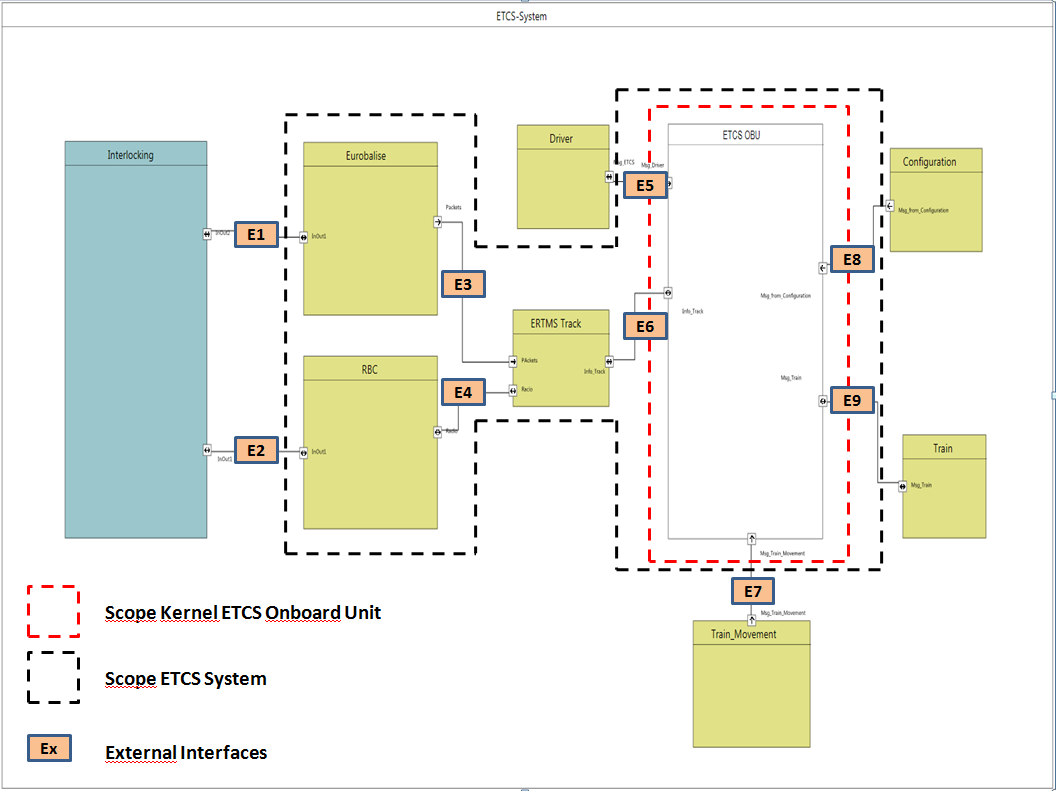
\includegraphics[scale=0.6]{images/1stlevelarchitecture}
\caption{1st level System Architecture view}
\label{1st level System Architecture view}
\end{figure}

\newpage
\subsection{2st level System Architecture view}
\textbf{The 2nd level system view will provide a decopmosition of the ETCS Onboard Unit systems and the Kernerl of the ETCS. The Kernel is the main part of the ETCS Onboard Unit system and reflects the functions specified in the ERA TSI Subset 26. Therefore the boundaries and interfaces to the other subasystems of the ETCS Onbard Unit needs to be fully desribed and formal. At least the formalisation kernel functions and boundaries should be realized in the openETCS project.}

\begin{figure}[h]
\centering
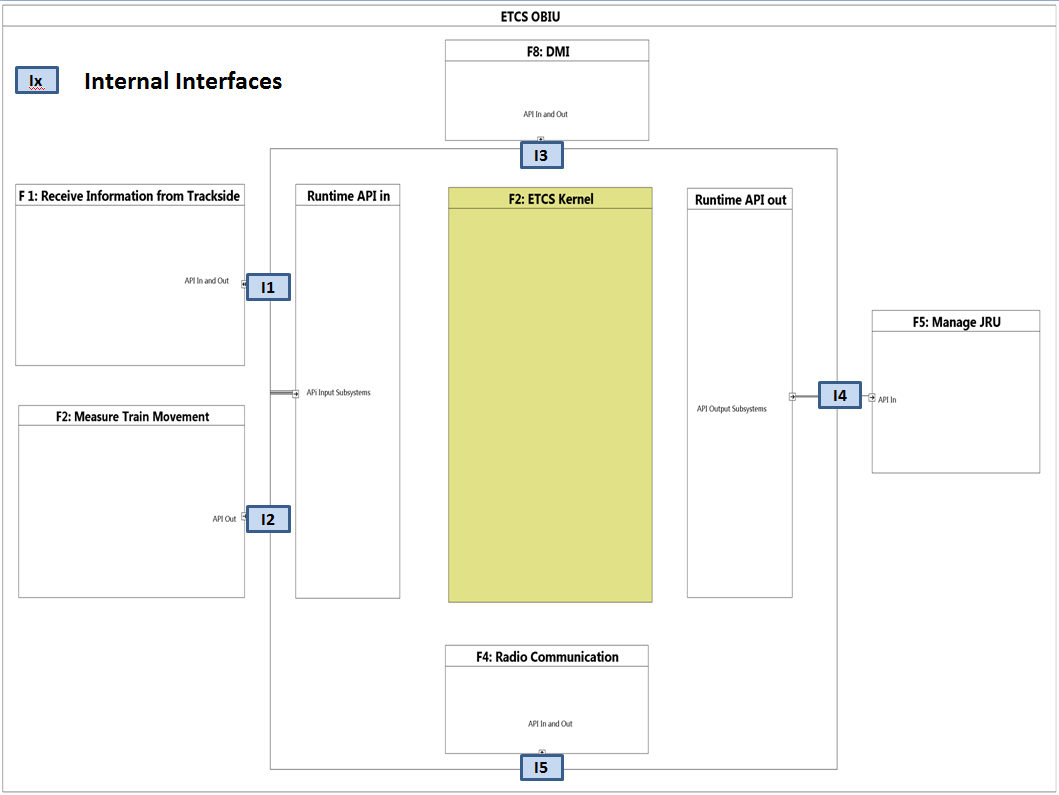
\includegraphics[scale=0.6]{images/2ndlevelarchitecture}
\caption{2nd level System Architecture view}
\label{2nd level System Architecture view}
\end{figure}

\subsection{3rd level System Architecture view}
\textbf{The 3rd level system view will provide a decopmosition of the ETCS Kernel of the ETCS Onboard Unit Systems. The decomposition and further design of the subfunctions of the kernel are part of the chapter 6 in this document. In chapter 6 we will consider the design description that will be completed by every designer itself. The designer can decided in this layer about the decomposition and boundaries of his subsystem, but need to describe the design choices.}

\newpage
\section{Interfaces}
\textbf{This section will consider the External and Internal interfaces as descibed in the system decomposition figures in 4.2.1 and 4.2.2}

\subsection{External Interfaces}
\textbf{External interfaces will describe the data flow between systems outside of the scope of the openETCS Project}

\paragraph*{E1: In- and Out flow between the Interlocking an Eurobalise. There will be 2 kind of balises}

\begin{itemize}
\item Fixed Balise: no interaction to the interlocking
\item Balise Controlled: interaction to the interlocking trough LEU
\end{itemize}

\begin{figure}[h]
\centering
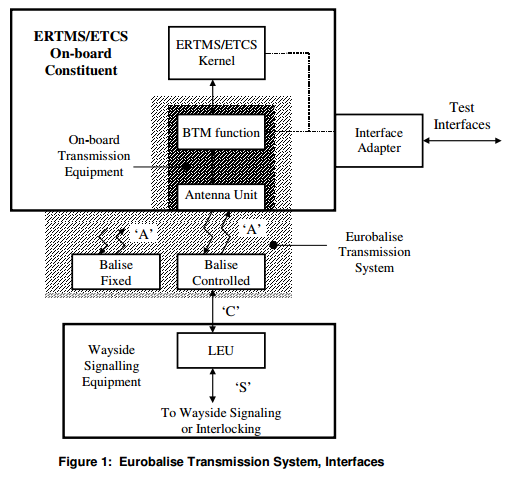
\includegraphics[scale=0.8]{images/Eurobalise}
\caption{Eurobalise}
\label{Eurobalise}
\end{figure}


\paragraph{E2: In- and Out flow between the Interlocking and Radio Block Control.}
This External interface will ensure the states or logics directly to the Radio Block Control and the other way back from the train to the interlocking.\\

\paragraph{E3:}

\paragraph{E4:}

\paragraph{E5:}

\paragraph{E6:}

\paragraph{E7:}

\paragraph{E8:}

\paragraph{E9:}

\subsection{Internal Interfaces}

\paragraph{I1:}

\paragraph{I2:}

\paragraph{I3:}

\paragraph{I4:}

\paragraph{I5:}



\chapter{Runtime API}

\section{Introduction to the Architecture}

\subsection{Abstract Hardware Architecture}

For proper understanding of openETCS API and of constraints imposed on
both sides of the API, we need to define a \emph{reference abstract hardware architecture}. This hardware architecture is ``abstract''
is the sense that the actual vendor specific hardware architecture
might be totally different of the abstract architecture described in
this chapter. For example, several units might be grouped together on
the same processor.

However, the actual vendor specific architecture shall fulfill all the
requirements and constraints of this reference abstract hardware
architecture and shall not request additional constraints.

\subsection{Definition of the Reference Abstract Hardware Architecture}

\begin{figure}
  \centering
  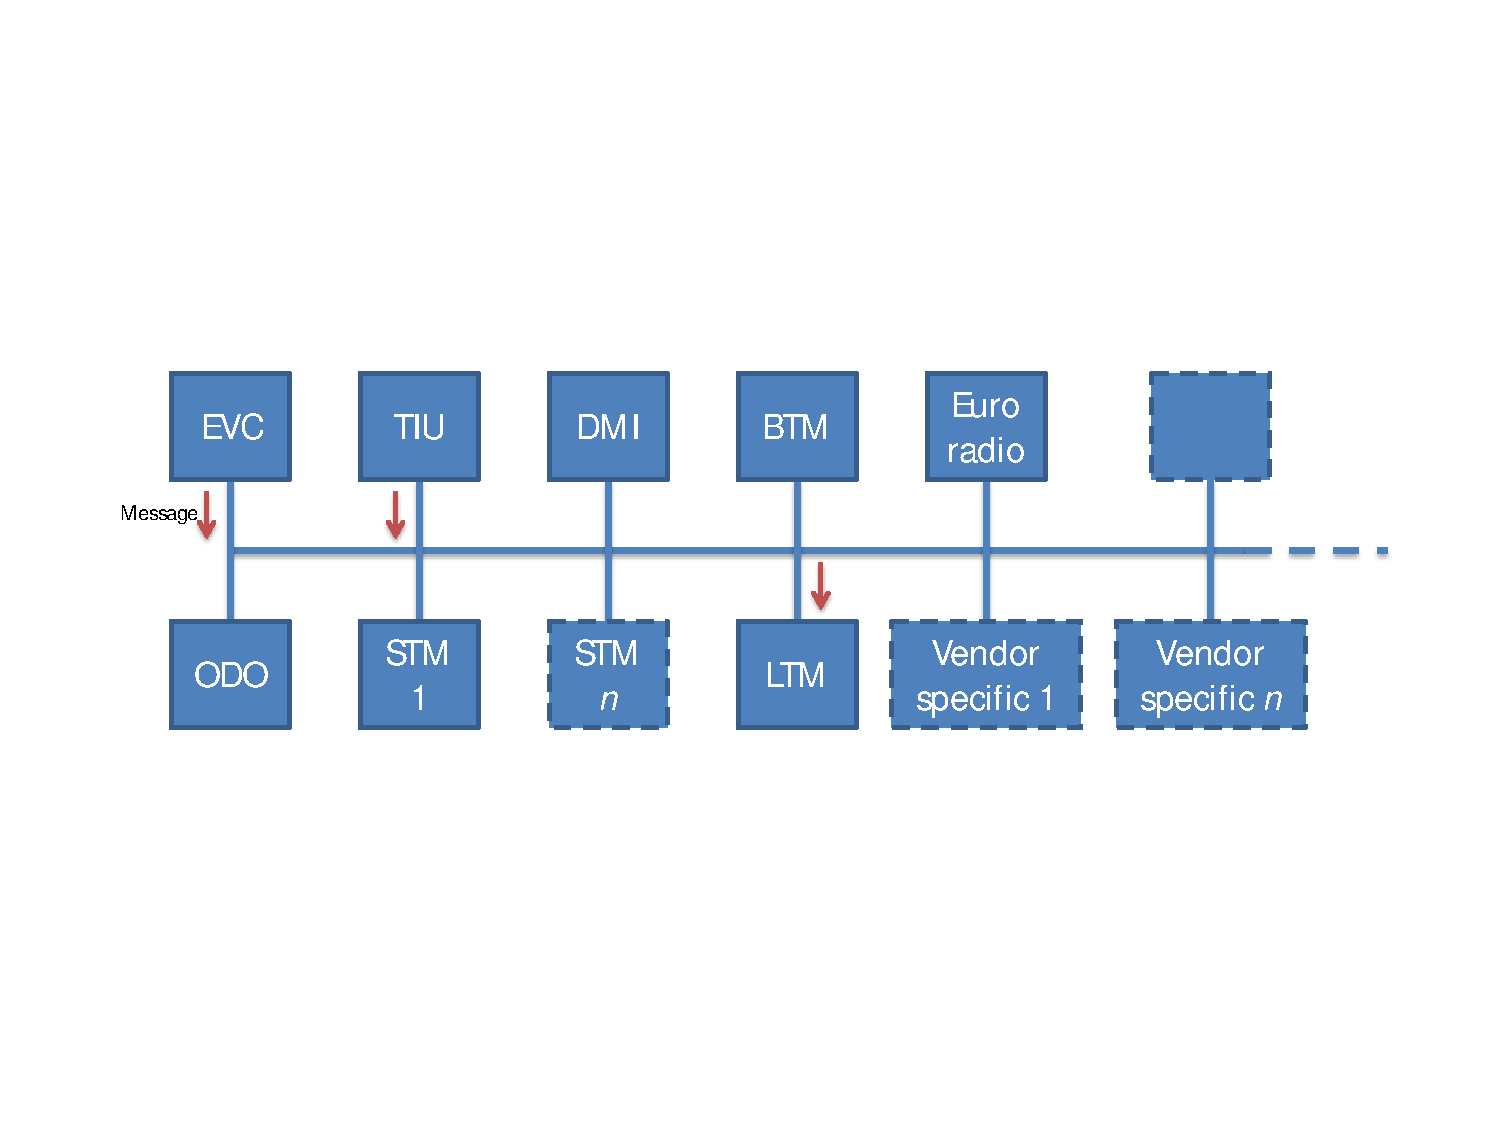
\includegraphics[width=\textwidth]{abstract-hardware-architecture.pdf}
  \caption{Reference abstract hardware architecture.}
  \label{fig:hardware-arch}
\end{figure}

The reference abstract hardware architecture is shown in Figure
\ref{fig:hardware-arch}. The reference abstract hardware architecture is made of a bus on which are connected \emph{units} defining the OBU:

\begin{itemize}
\item {EVC};
\item {TIU};
\item {ODO};
\item {DMI};
\item {STM};
\item {BTM};
\item {LTM}: Not part of this openETCS implementation;
\item EURORADIO;
\item {JRU}: Not part of this openETCS implementation;
\end{itemize}

Elements not being part of this implementation are marked. Those units shall working concurrently. They shall exchange information with other units through asynchronous message passing.

\subsection{Reference abstract software architecture}
\label{software-arch}

\begin{figure}
  \centering
  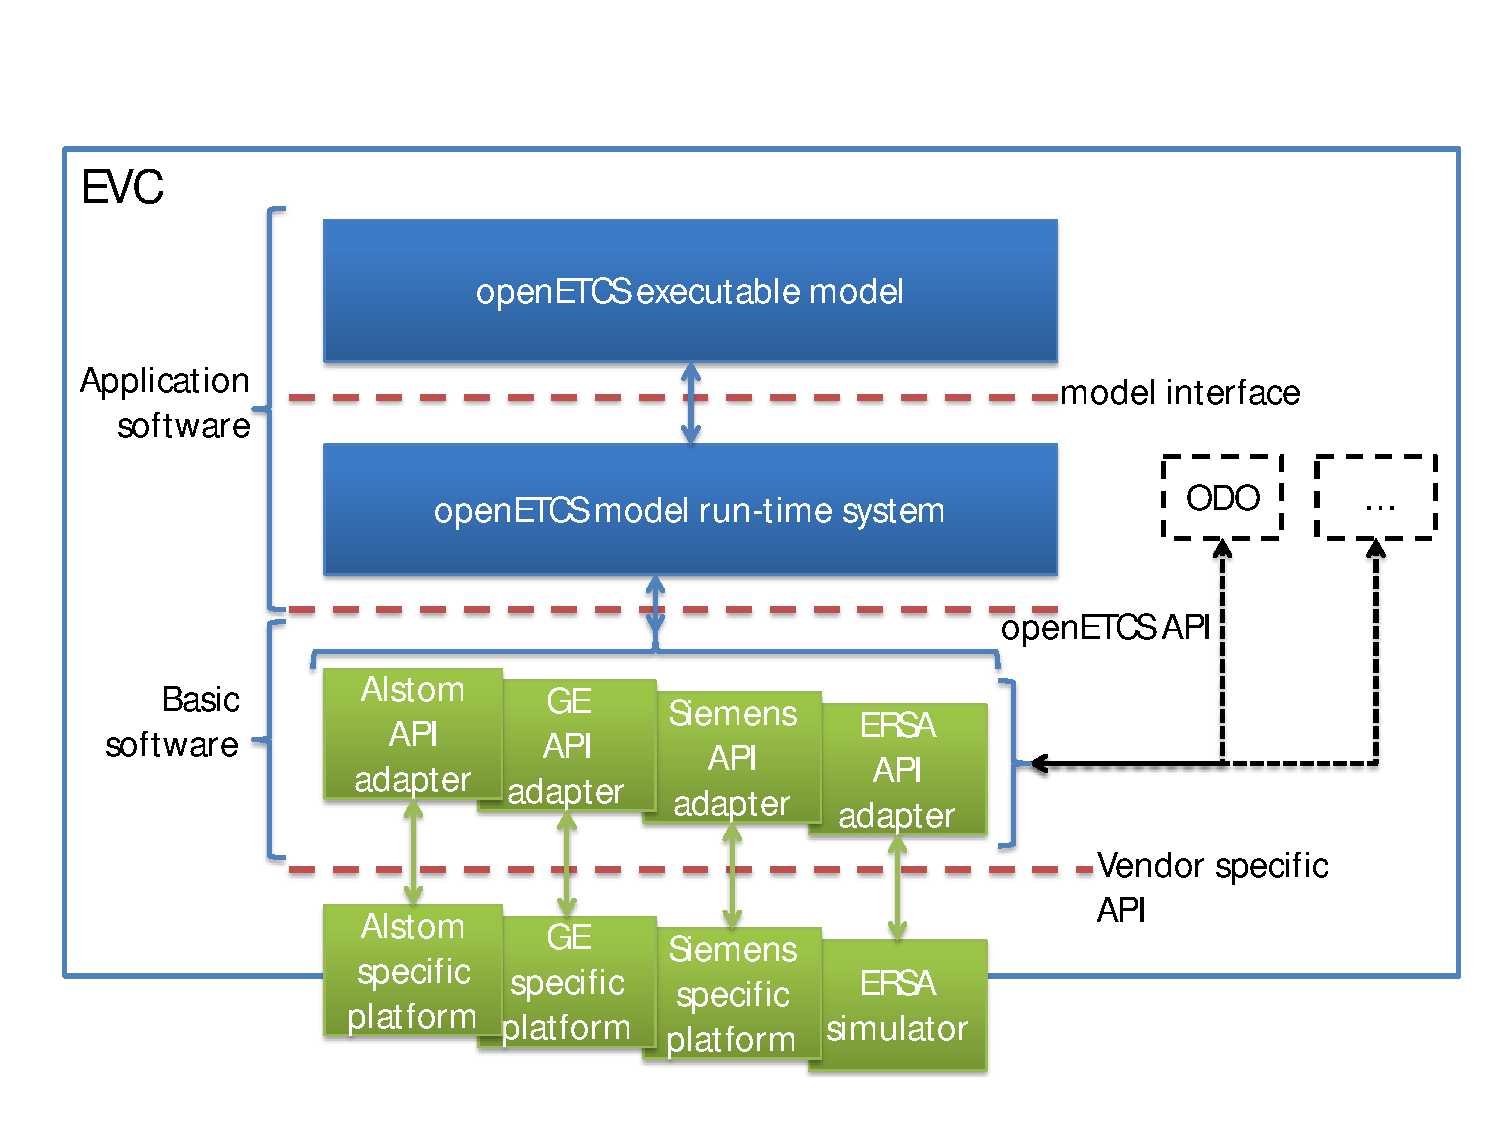
\includegraphics[width=0.9\textwidth]{software-architecture.pdf}
  \caption{Reference abstract software architecture}
  \label{fig:software-arch}
\end{figure}

The \emph{reference abstract software architecture} is shown in Figure
\ref{fig:software-arch}. This architecture consists of following
elements:
\begin{description}
\item[openETCS executable model] produced by the SCADE model \cite{scade-model}. It shall contain the program implementing core
  ETCS functions;
\item[openETCS model run-time system] shall help the execution
  of the openETCS executable model by providing additional functions
  like encode/decode messages, proper execution of the model through
  appropriate scheduling, re-order or prioritize messages, etc. 
\item[Vendor specific API adapter] shall make the link between
  the Vendor specific platform and the openETCS model run-time system.
  It can buffer message parts, encode/decode messages, route messages
  to other EVC components, etc.
\item[EVC] All above three elements shall be included in the EVC;
\item[Vendor specific platform] shall be all other elements of
  the system, bus and other units, as shown in Figure \ref{fig:hardware-arch}.
\end{description}

We have thus three interfaces:
\begin{description}
\item[Model interface]
 is the interface between openETCS executable model and openETCS model run-time system. 
\item[openETCS {API}]
 is the interface between openETCS model run-time system and Vendor specific {API} adapter.
\item[Vendor specific {API}]
 is the interface between Vendor specific {API} adapter and Vendor specific platform. This interface is not publicly described for all vendors. You can find the Alstom implementation as an example.
\end{description}

The two blocks openETCS executable model and openETCS model run-time
system are making the \emph{application software} part. This application software might be either openETCS reference software or vendor specific software.

The Vendor specific API adapter is making the \emph{Basic software} part.







\bibliographystyle{unsrt}
\bibliography{architecture}


\addcontentsline{toc}{chapter}{Index}
\printindex
%===================================================
%Do NOT change anything below this line

\end{document}
